\documentclass{article}
\usepackage{pgfplots}
\pgfplotsset{compat=1.18}

\begin{document}

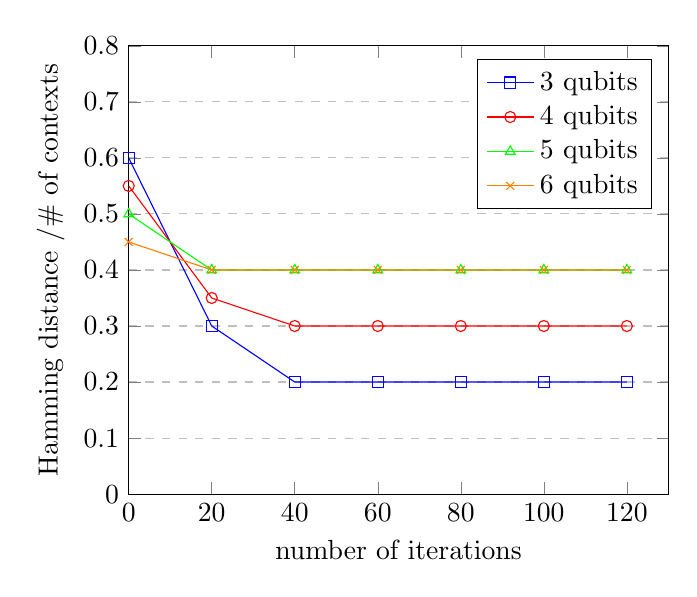
\begin{tikzpicture}
    \begin{axis}[
        xlabel={number of iterations},
        ylabel={Hamming distance /$\#$ of contexts},
        xmin=0, xmax=130,
        ymin=0, ymax=0.8,
        xtick={0,20,...,120},
        ytick={0,0.1,...,0.8},
        legend pos=north east,
        ymajorgrids=true,
        grid style=dashed,
    ]
    
    % Data for 3 qubits
    \addplot[
        color=blue,
        mark=square,
        ]
        coordinates {
            (0,0.6)
            (20,0.3)
            (40,0.2)
            (60,0.2)
            (80,0.2)
            (100,0.2)
            (120,0.2)
        };
        \addlegendentry{3 qubits}
        
    % Data for 4 qubits
    \addplot[
        color=red,
        mark=o,
        ]
        coordinates {
            (0,0.55)
            (20,0.35)
            (40,0.3)
            (60,0.3)
            (80,0.3)
            (100,0.3)
            (120,0.3)
        };
        \addlegendentry{4 qubits}
        
    % Data for 5 qubits
    \addplot[
        color=green,
        mark=triangle,
        ]
        coordinates {
            (0,0.5)
            (20,0.4)
            (40,0.4)
            (60,0.4)
            (80,0.4)
            (100,0.4)
            (120,0.4)
        };
        \addlegendentry{5 qubits}
        
    % Data for 6 qubits
    \addplot[
        color=orange,
        mark=x,
        ]
        coordinates {
            (0,0.45)
            (20,0.4)
            (40,0.4)
            (60,0.4)
            (80,0.4)
            (100,0.4)
            (120,0.4)
        };
        \addlegendentry{6 qubits}
        
    \end{axis}
\end{tikzpicture}

\end{document}